\chapter{Theory}
\label{ch:theory}
A radio telescope measures the power it receives as a function of frequency
and time. In this chapter we first describe what this data looks like and how
RFI appears in it, and then the neural network, loss functions and evaluation
measures that are used in the rest of this work.

\section{Radio Spectrograms and Noise}
After the signal from a radio telescope is split into frequency channels, the
data can be written as a spectrogram, also called a dynamic spectrum. Each
pixel holds the power received in one frequency channel during one short time
interval. Even when no astronomical source is present, every pixel contains
noise from the receiver electronics and from the sky. This noise is thermal in
origin and, because it is the sum of many independent contributions, it
follows a Gaussian distribution. Its level is given by the radiometer
equation\footcite{wilson2013tools}:
\begin{equation}
  \sigma_T = \frac{T_{\text{sys}}}{\sqrt{\Delta\nu\,\tau}}
  \label{eq:radiometer}
\end{equation}
where $T_{\text{sys}}$ is the system temperature, $\Delta\nu$ is the channel
bandwidth and $\tau$ is the integration time. Averaging over more bandwidth or a
longer time therefore lowers the noise. For the same reason, a faint signal
that extends over many pixels can still be detected even when each single
pixel lies below the noise.

The receiver also does not amplify every frequency by the same amount. Its gain
falls off at the edges of the observing band and has small ripples across it.
This frequency-dependent gain is called the bandpass. It adds smooth structure
to every spectrogram, which a flagging method must not mistake for RFI.

\section{Radio Frequency Interference}
\label{sec:rfi_types}
Unlike the noise, RFI is non-Gaussian and non-stationary. Different kinds of
RFI leave different shapes in a spectrogram, depending on how long they last
and how many frequencies they cover. \Cref{fig:rfi_types} shows these types of
RFI in a real observation.

\begin{figure}[H]
  \centering
  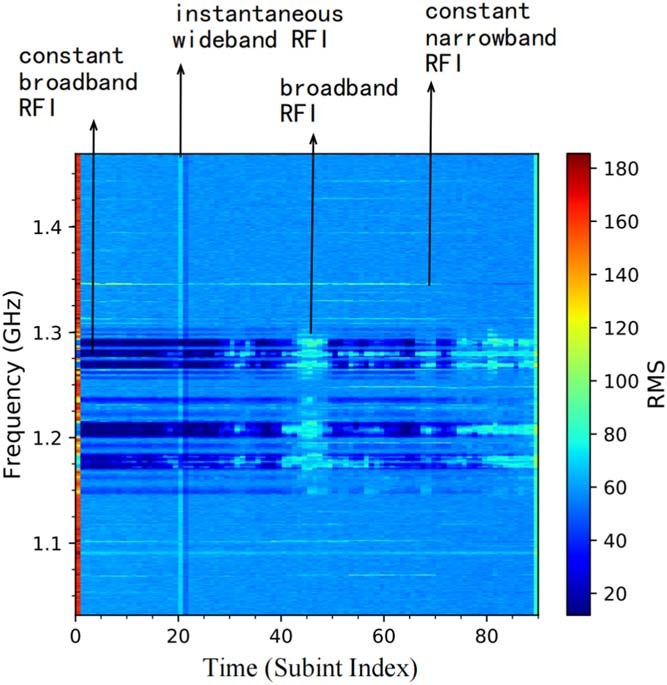
\includegraphics[width=0.62\textwidth]{chen2023_fig1_rfi_types}
  \caption[Types of RFI in a real observation]{Types of RFI in folded pulsar
    data observed with the FAST telescope (PSR J1859+0430): constant broadband
    RFI from satellites, instantaneous wideband RFI, broadband RFI lasting a few
    minutes, and constant narrowband RFI. The colour shows the rms of the folded
    pulse profile in each frequency channel and sub-integration. Reproduced from
    Chen et al.\ (2023).}
  \label{fig:rfi_types}
\end{figure}

\begin{itemize}
  \item \textbf{Constant narrowband RFI} affects a single frequency channel for
    the whole observation and appears as a thin line along the time axis.
    Fixed terrestrial transmitters are a typical source.
  \item \textbf{Constant broadband RFI} covers a wide range of frequencies for
    the whole observation and appears as a thick band, for example from
    continuously broadcasting satellites.
  \item \textbf{Instantaneous wideband RFI} lasts only a moment but covers
    almost all frequencies, appearing as a thin line along the frequency axis.
    Lightning, arcing on power lines and radar produce this kind.
  \item \textbf{Patchy broadband RFI} covers several channels for a few minutes
    and then fades, appearing as irregular, cloud-like patches.
\end{itemize}



\section{Classical Flagging Methods}
The simplest way to flag RFI is to mark every pixel whose value $x$ lies too
far from the typical value of the data:
\begin{equation}
  |x - \mu| > k\,\sigma
  \label{eq:threshold}
\end{equation}
where $\mu$ and $\sigma$ are the mean and standard deviation of the data (or
robust versions of them such as the median) and $k$ is chosen by the user.
Tools for folded pulsar data such as \texttt{paz} and \texttt{clfd} work in this
way. They need no training, but they assume that the clean data is Gaussian, so
they miss faint RFI and struggle when the noise level changes across the data.

\aoflagger{}\footcite{offringa2012} is the standard RFI flagger for LOFAR. It
looks for unusually bright pixels at several scales, and then grows each
flagged region a little along time and frequency so that the faint edges of the
RFI are flagged too. It is important for this work because it produced the training labels
of the LOFAR dataset.

\section{Convolutional Neural Networks}
A convolutional neural network (CNN) processes an image with small learned
filters. A convolutional layer slides a filter $w$ of size $M \times N$ over the
input $x$ and computes, at every position,
\begin{equation}
  y(i,j) = \sum_{m=1}^{M}\sum_{n=1}^{N} w(m,n)\,x(i+m,\,j+n) + b
  \label{eq:conv}
\end{equation}
where $b$ is a learned bias. The result is passed through a non-linear
activation function, most commonly the rectified linear unit,
$\mathrm{ReLU}(z) = \max(0, z)$. Stacking many such layers lets the network
build up complex features from simple ones. Pooling layers halve the size of
the image between some of the layers, so that later filters see a larger part
of the input. The filter weights are learned by gradient descent, which changes
them step by step to reduce a loss function that measures how wrong the
network's output is. In this work we use the Adam
optimiser\footcite{kingma2015adam}, a variant of gradient descent that adapts
the step size for each weight.

\section{The U-Net Architecture}
\label{sec:unet}
The U-Net\footcite{ronneberger2015} is a CNN designed for image segmentation
(\cref{fig:unet}). Its encoder, the downsampling path, repeatedly applies
convolutions and halves the image size, building up a description of
\emph{what} is in the image. Its decoder, the upsampling path, reverses this
and restores the full size to locate \emph{where} it is. Skip connections pass
fine detail directly from each encoder level to the matching decoder level,
where it is joined (concatenated) with the upsampled features. In the original
network each level uses two 3$\times$3 convolutions with ReLU, the image is
halved by 2$\times$2 max pooling and doubled again by 2$\times$2 up-convolutions,
and a final 1$\times$1 convolution gives the class scores. For every pixel
the last layer produces one score $z_c$ for each class $c$, here ``clean'' and
``RFI'', and these scores are turned into probabilities by the softmax function:
\begin{equation}
  p_c = \frac{e^{z_c}}{\sum_k e^{z_k}}
  \label{eq:softmax}
\end{equation}

\begin{figure}[H]
  \centering
  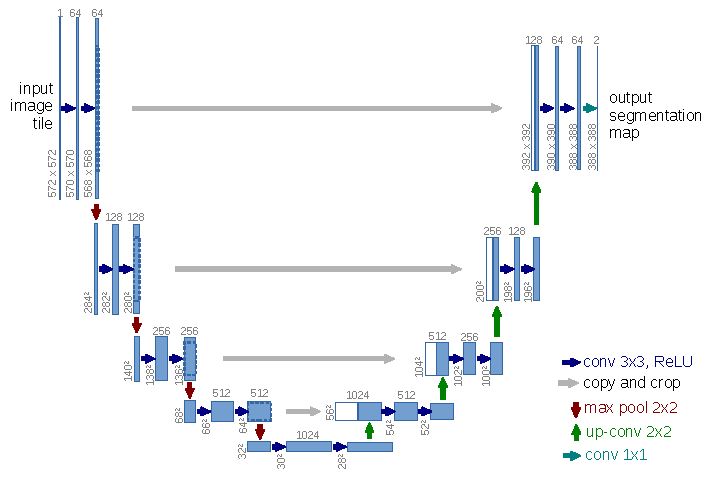
\includegraphics[width=0.9\textwidth]{ronneberger2015_unet_fig1}
  \caption[The U-Net architecture]{The U-Net architecture (example for
    32$\times$32 pixels at the lowest resolution). Each blue box is a
    multi-channel feature map, with the number of channels on top and the size
    at its lower left; white boxes are copied feature maps, and the arrows mark
    the operations. Reproduced from Ronneberger et al.\ (2015).}
  \label{fig:unet}
\end{figure}

Akeret et al.\footcite{akeret2017} applied a U-Net to RFI in their \tfunet{}
code, written in TensorFlow (\cref{fig:tfunet_arch}). The configuration used in this work has 3 levels
and 32 filters in the first layer, giving 465{,}986 trainable parameters. Two
details of \tfunet{} become important later: it applies a ReLU to its output
scores before the softmax, and it has no normalisation layers.

\section{Loss Functions}
\label{sec:losses}
The most common loss for segmentation is the cross-entropy. If $p_{i}$ is the
predicted probability of the correct class $y_i$ for pixel $i$, the weighted
cross-entropy is
\begin{equation}
  L_{\text{CE}} = -\frac{\sum_i w_{y_i} \log p_{i}}{\sum_i w_{y_i}}
  \label{eq:ce}
\end{equation}
where $w_{y_i}$ is the weight of the class of pixel $i$. With all weights equal
to one this is the plain cross-entropy. When one class is much rarer than the
other, as RFI is, the rare class is sometimes given a larger weight, which is
called class weighting.

The Dice loss\footcite{milletari2016} instead measures how well the predicted
RFI region overlaps the true one as a whole:
\begin{equation}
  L_{\text{Dice}} = 1 - \frac{2\sum_i p_i g_i + \epsilon}{\sum_i p_i + \sum_i g_i + \epsilon}
  \label{eq:dice}
\end{equation}
where $p_i$ is the predicted RFI probability of pixel $i$, $g_i$ is 1 if the
pixel is labelled RFI and 0 otherwise, and $\epsilon = 1$ avoids division by
zero. Because it depends only on the RFI pixels, it is not dominated by the
large number of clean pixels.

\section{Evaluation Metrics}
\label{sec:metrics}
For each pixel, a flagging method either flags it as RFI or not, and the pixel
either is or is not RFI in the reference labels. Counting the true positives
(TP), false positives (FP) and false negatives (FN) gives
\begin{equation}
  \text{precision} = \frac{TP}{TP + FP}, \qquad
  \text{recall} = \frac{TP}{TP + FN}, \qquad
  F_1 = \frac{2\,\text{precision}\cdot\text{recall}}{\text{precision} + \text{recall}}
  \label{eq:f1}
\end{equation}
Precision is the fraction of flagged pixels that really are RFI, and recall is
the fraction of the RFI that was found. \Fone{} is high only if both are.
Accuracy, the fraction of pixels classified correctly, is not useful here: RFI
covers less than 1\% of the LOFAR test pixels, so a method that flags nothing
at all is 99.23\% accurate while finding no RFI. The area under the ROC curve
(ROC AUC) measures something different, namely how well a model \emph{ranks} RFI
pixels above clean ones, regardless of where the final cut is made.

A network outputs a probability for each pixel, and a threshold turns it into a
yes/no decision. We report \Fone{} in two ways:
\begin{itemize}
  \item \textbf{Maximum \Fone{}:} every threshold is tried on the test set and
    the best is reported. This is optimistic, because it uses the test labels
    to pick the threshold, but it is the measure used in the published LOFAR
    results, so it is needed for a fair comparison with them.
  \item \textbf{Pooled \Fone{}:} the threshold is chosen on a separate
    validation set and then applied to the test set. This is the honest
    measure of how a model would perform on new data.
\end{itemize}
